\section{Input \& Output} \label{sec:input-output}

\begin{multicols}{2}

\begin{figure}[H]
    \centering
    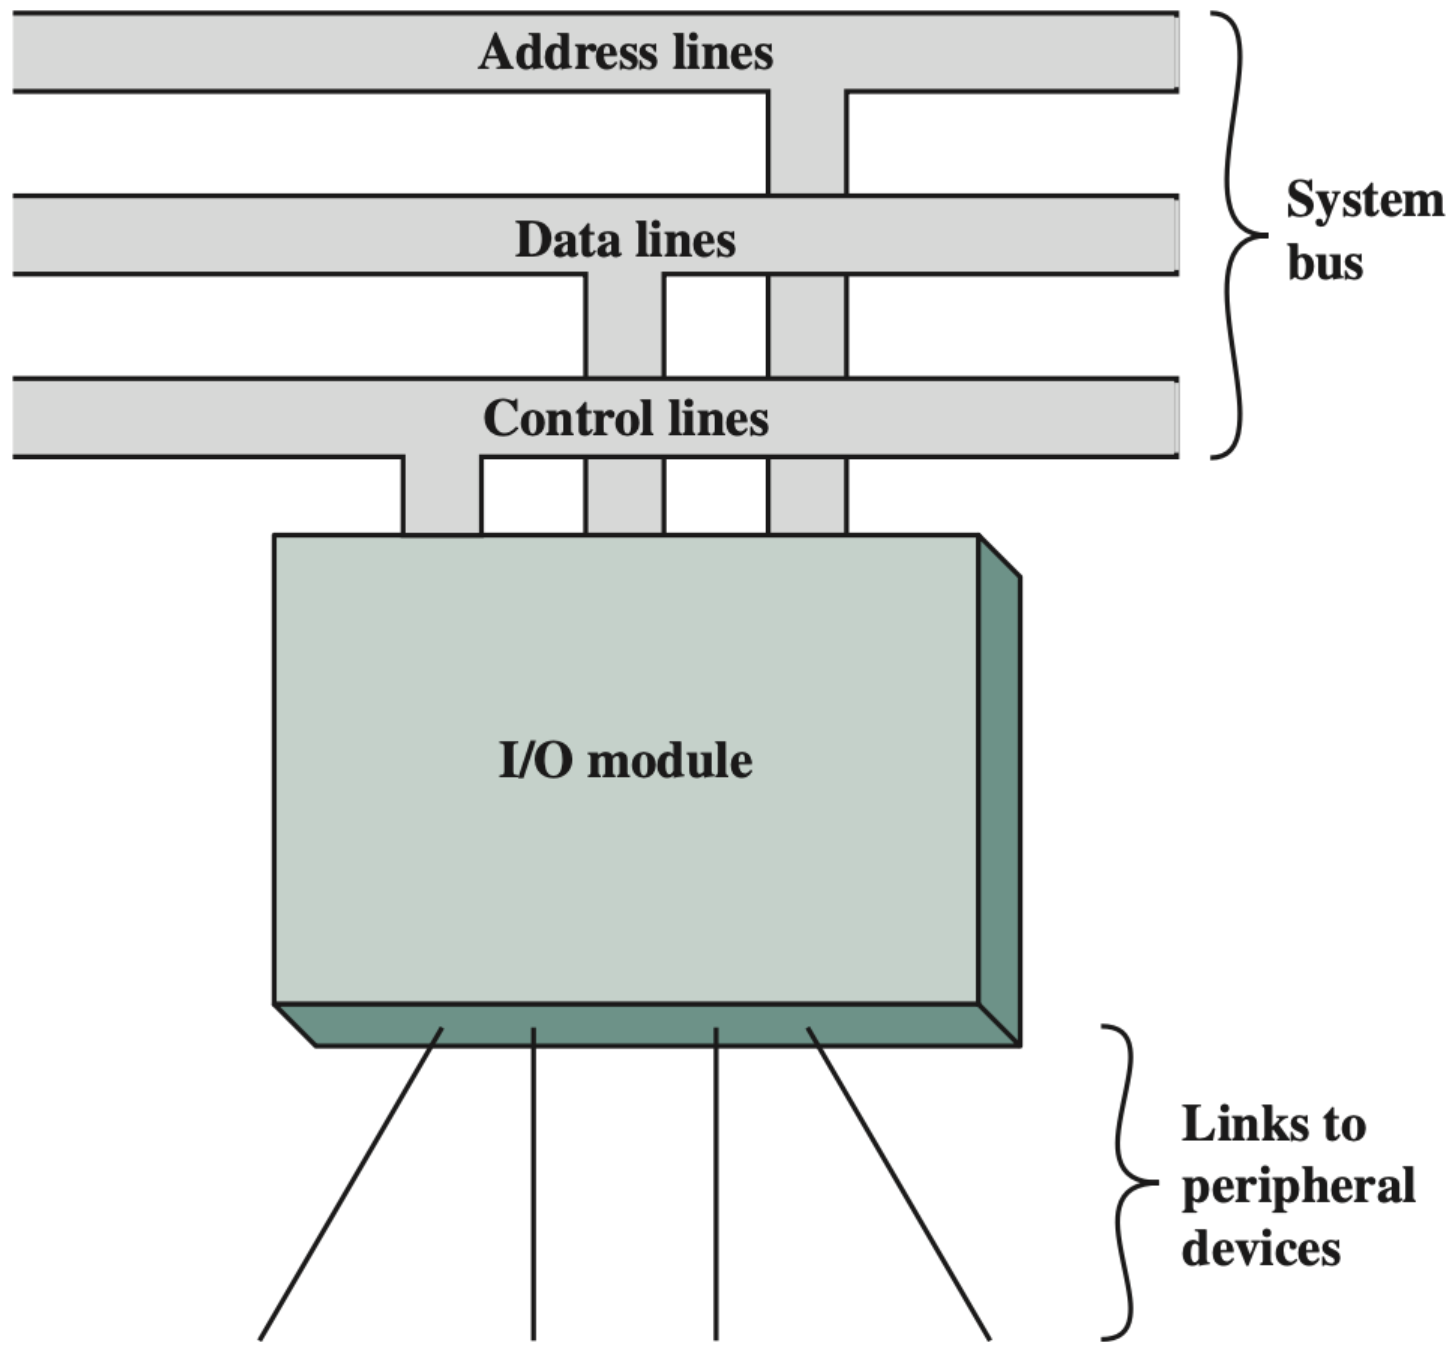
\includegraphics[width=\linewidth]{chaps/input-output/io-module-model.png}
    \caption{Generic Model of an I/O Module}
\end{figure}

\columnbreak

\subsection{Generic Model of I/O Modules}

An I/O module is:
\begin{itemize}
    \item an interface between the processor and memory via the system bus or central switch
    \item an interface to one ore more peripheral devices through tailored data links
\end{itemize}

Major requirements on an I/O module:
\begin{itemize}
    \item \textbf{Asynchronous timing}.
    \item \textbf{Command decoding}: interpret the commands sent from the bus, e.g. \texttt{SEEK}.
    \item \textbf{Data}: exchange data via the data bus.
    \item \textbf{Status reporting}: e.g. Ready, Busy, Out of Paper (printer).
    \item \textbf{Address recognition}: identify the address of a peripheral device.
    \item \textbf{Data buffering}: for speeding up transaction because the device may be slower.
    \item \textbf{Error detection and correction}.
\end{itemize}

\end{multicols}

The CPU operates I/O devices by reading/writing from/to the devices' status/control/data
registers. The registers are mapped in two ways:
\begin{enumerate}
    \item \textbf{Memory-mapped I/O}: the I/O device registers are mapped into the same
        address space as the memory. The CPU can access the I/O device registers as if
        they were memory locations.
    \item \textbf{Port-mapped I/O}: the I/O device registers are mapped into a separate
        address space from the memory. The CPU uses special I/O instructions to access
        the I/O device registers. \label{lbl:port-mapped-io}
\end{enumerate}

\subsection{I/O Techniques}

Three types of I/O techniques for interacting with I/O devices:
\begin{itemize}
    \item Not using interrupts: \textbf{Programmed I/O}
    \item Using interrupts: \begin{itemize}
        \item \textbf{Interrupt-driven I/O} (Memory $\leftrightarrow$ CPU $\leftrightarrow$ I/O)
        \item \textbf{Direct Memory Access (DMA)} (Memory $\leftrightarrow$ I/O)
    \end{itemize}.
\end{itemize}

\begin{figure}[htb]
    \centering
    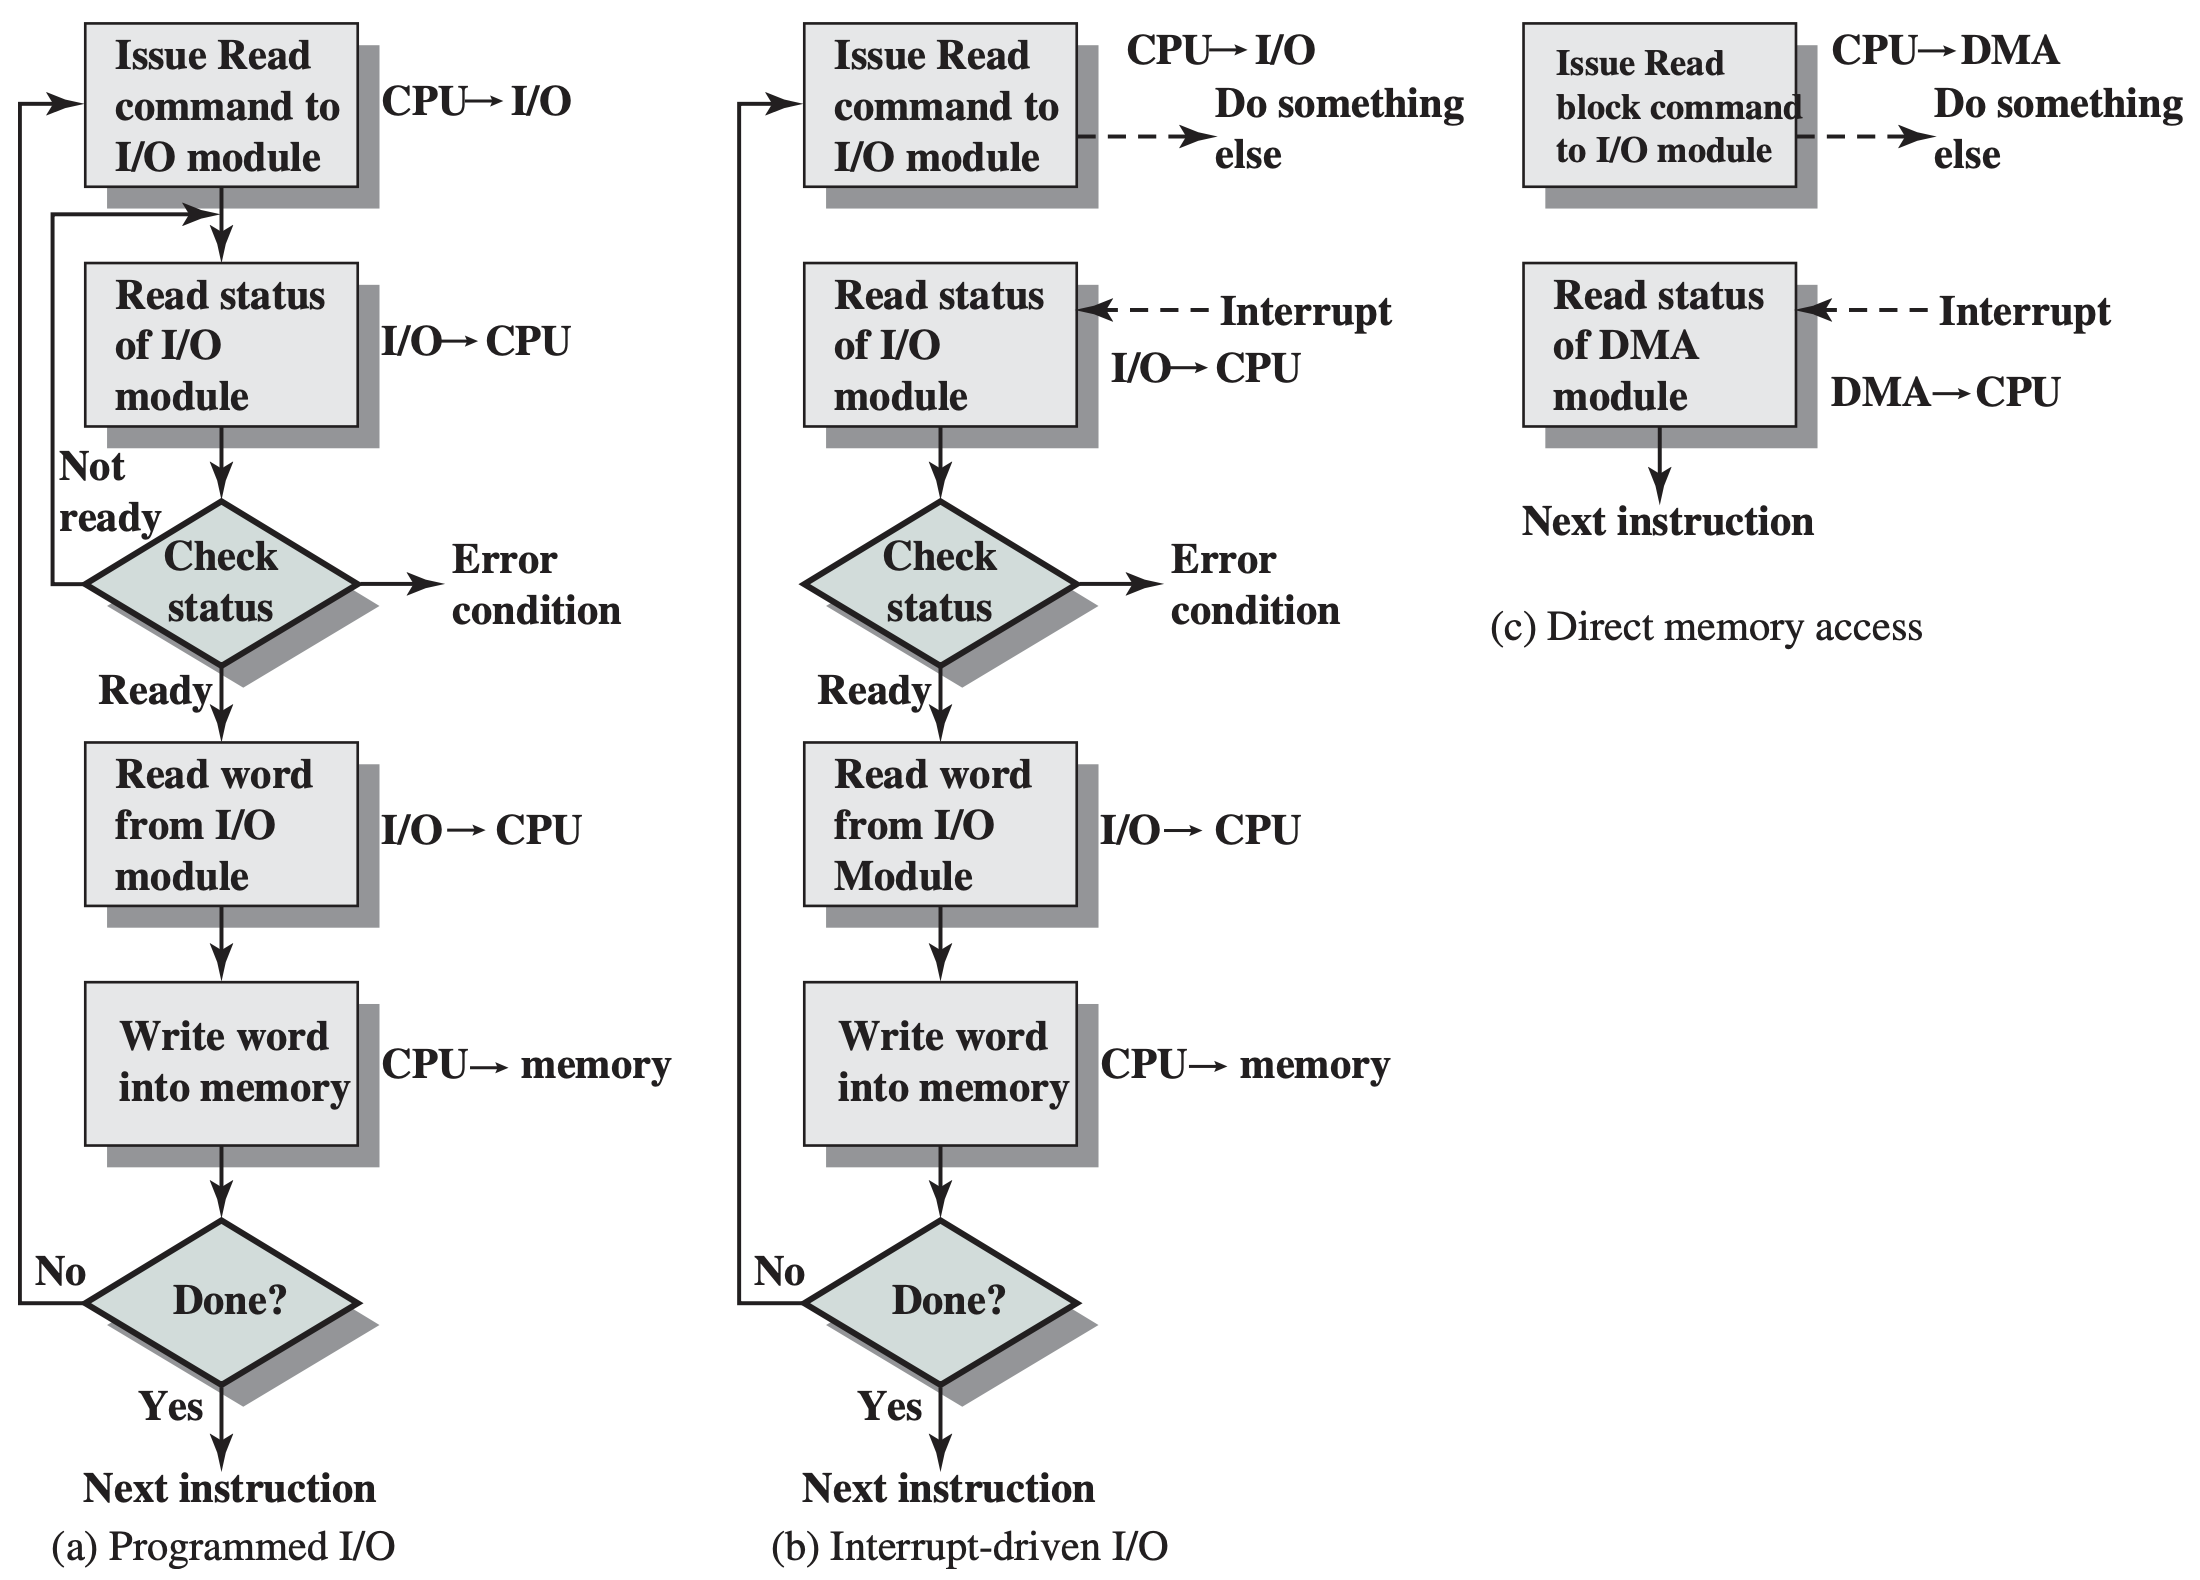
\includegraphics[width=0.9\linewidth]{chaps/input-output/io-techniques.png}
    \caption{I/O Techniques}
\end{figure}

\subsubsection{Programmed I/O}

The processor executes a program to control the I/O devices via the Control and Status
Registers (CSR). When the CPU sends a command
to the device, it must wait for the device to complete. This wastes CPU time.

\subsubsection{Interrupt-Driven I/O}

This technique attempts to alleviate the issues of Programmed I/O. After sending a command
to the I/O module, the CPU will carry on with other tasks. When the I/O module finishes,
it sends an interrupt signal to the CPU. The CPU will then handle the interrupt and return
to its tasks.

The CPU sends a interrupt acknowledge signal (\texttt{INTA}) to the I/O module to indicate
receipt of the interrupt signal. The last instruction of the interrupt routine is a return
from interrupt instruction (\texttt{RETI}). Refer to Section \ref{subsubsec:interrupts} for
interrupt handling procedures.

\subsubsection{Direct Memory Access (DMA)}

Interrupt-Driven I/O still involves CPU operations, which can be minimised by a special
purpose processor -- \textbf{Input-Output Processor (IOP)}.

To resolve bus conflicts between the CPU and IOP, the IOP steals cycles from the CPU by
sending a signal to the CPU. The CPU will now see an elongated clock cycle, and will wait
until the cycle ends to continue.

\textbf{Difference between Interrupt-Driven I/O and DMA}: The ``interruption'' in DMA is
\textbf{within} one instruction execution cycle, while the interruption in Interrupt-Driven
I/O is after the instruction execution cycle, as illustrated in Figure
\ref{fig:interrupt-driven-io-vs-dma}.

\begin{figure}[H]
    \centering
    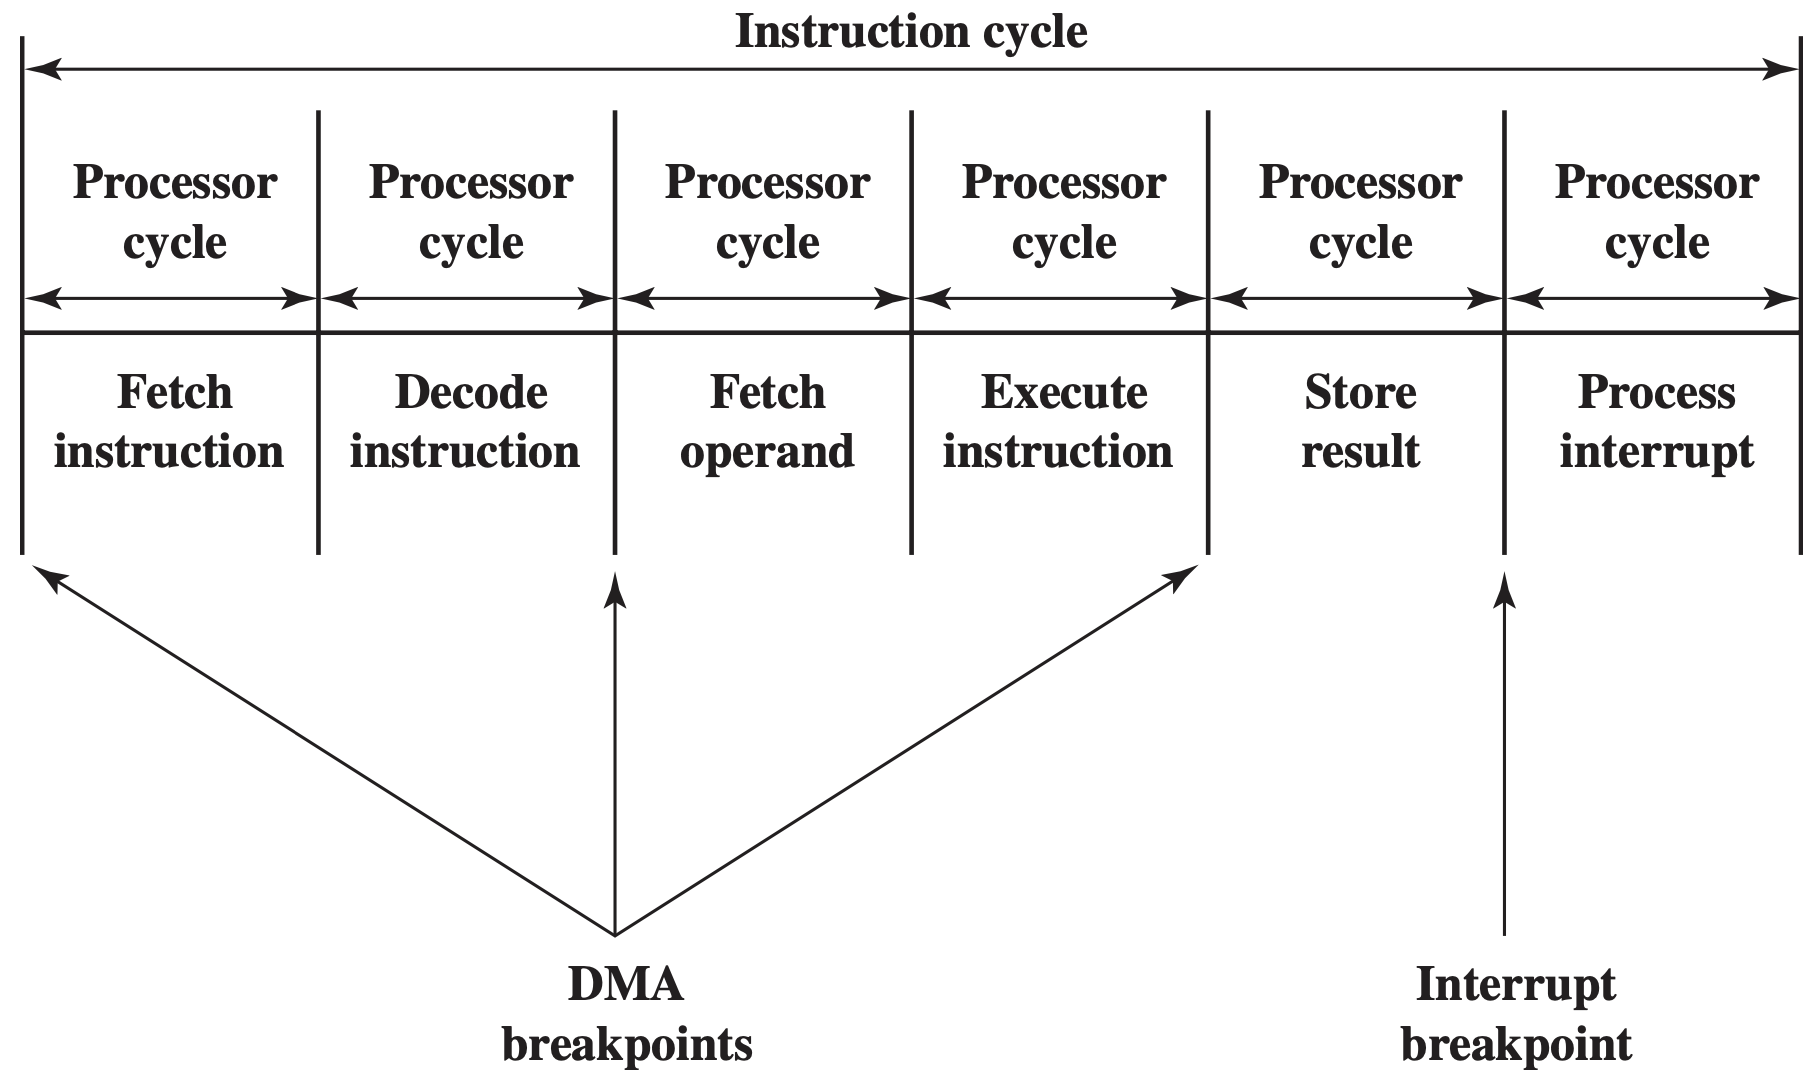
\includegraphics[width=0.6\textwidth]{chaps/input-output/interrupt-driven-io-vs-dma.png}
    \caption{Difference between Interrupt-Driven I/O and DMA}
    \label{fig:interrupt-driven-io-vs-dma}
\end{figure}